\documentclass[11pt,aspectratio=169]{beamer}

% -------------------- THEME & LAYOUT --------------------
\usetheme{Madrid}
\usecolortheme{dolphin}
\usefonttheme{professionalfonts}
\setbeamercovered{transparent}
\setbeamertemplate{navigation symbols}{}
\setbeamertemplate{caption}[numbered]
\setbeamertemplate{itemize items}[triangle]
\setbeamersize{text margin left=1.2cm,text margin right=1.2cm}

% -------------------- GLOBAL FONT SETTINGS --------------------
\setbeamerfont{normal text}{size=\small}
\setbeamerfont{math text}{size=\small}
\setbeamerfont{equation}{size=\small}
\let\oldnormalsize\normalsize
\renewcommand{\normalsize}{\oldnormalsize\small}
\setbeamerfont{itemize/enumerate body}{size=\small}
\setbeamerfont{itemize/enumerate subbody}{size=\small}

% -------------------- FONTS & TYPOGRAPHY --------------------
\usepackage[T1]{fontenc}
\usepackage[utf8]{inputenc}
\usepackage{newpxtext,newpxmath}
\usepackage{microtype}

% -------------------- MATH, TABLES & GRAPHICS --------------------
\usepackage{amsmath,amssymb,amsfonts,mathtools}
\usepackage{bm,booktabs,siunitx,graphicx}
\graphicspath{{./}{./figures/}}
\usepackage{epstopdf}

% Numbered equations (Chapter 12)
\setcounter{equation}{0}
\renewcommand{\theequation}{12.\arabic{equation}}

% -------------------- UTILITIES --------------------
\usepackage{appendixnumberbeamer}
\usepackage{ragged2e}
\usepackage{xspace}
\usepackage{csquotes}
\usepackage{xcolor}
\usepackage{hyperref}
\usepackage[export]{adjustbox}

% -------------------- COLORS & EMPHASIS --------------------
\definecolor{myblue}{RGB}{0,70,140}
\definecolor{myred}{RGB}{180,30,30}
\definecolor{mygreen}{RGB}{0,120,70}
\definecolor{gold}{RGB}{184,134,11}

\setbeamercolor{title}{fg=gold}
\setbeamercolor{frametitle}{fg=gold}
\setbeamercolor{structure}{fg=gold}
\setbeamercolor{section in head/foot}{fg=gold,bg=black!10}

\newcommand{\highlight}[1]{\textcolor{myblue}{#1}}
\newcommand{\warning}[1]{\textcolor{myred}{#1}}

% -------------------- FOOTLINE --------------------
\setbeamertemplate{footline}{
  \leavevmode%
  \hbox{%
    \begin{beamercolorbox}[wd=0.7\paperwidth,ht=2.5ex,dp=1.5ex,leftskip=1.4em]{section in head/foot}%
      \ifx\insertsection\empty
      \else
        Section: \insertsection
      \fi
    \end{beamercolorbox}%
    \begin{beamercolorbox}[wd=0.3\paperwidth,ht=2.5ex,dp=1.5ex,leftskip=3.8cm]{section in head/foot}%
      \insertframenumber/\inserttotalframenumber
    \end{beamercolorbox}%
  }%
  \vskip1pt%
}

% -------------------- TIGHTER DISPLAY MATH --------------------
\makeatletter
\g@addto@macro\normalsize{%
  \setlength\abovedisplayskip{8pt}%
  \setlength\belowdisplayskip{8pt}%
  \setlength\abovedisplayshortskip{6pt}%
  \setlength\belowdisplayshortskip{6pt}%
}
\makeatother

\setbeamertemplate{frametitle}{
  \nointerlineskip
  \begin{beamercolorbox}[wd=\paperwidth,ht=3.5ex,dp=1ex,center]{frametitle}
    \centering\insertframetitle
  \end{beamercolorbox}
}

% -------------------- SHORTCUTS --------------------
\newcommand{\E}{\mathbb{E}}
\newcommand{\R}{\mathbb{R}}
\newcommand{\mc}[1]{\mathcal{#1}}
\newcommand{\bb}[1]{\mathbb{#1}}

% -------------------- METADATA --------------------
\title[Chapter 12 — Phillips Curve]{\textbf{Monetary Economics and Policy}\\[2pt]\large Chapter 12 — The Inflation Unemployment Trade Off}
\author{Pierpaolo Benigno}
\institute{}
\date{\today}

% -------------------- SECTION ROADMAP --------------------
\AtBeginSection[]
{
  \begin{frame}
    \tableofcontents[currentsection, hideothersubsections]
  \end{frame}
}

% -------------------- Bibliography --------------------
\usepackage[backend=biber,style=apa]{biblatex}
\addbibresource{sources.bib}

\begin{document}

% ===================== TITLE SLIDE =====================
\begin{frame}[plain] % 'plain' removes header/footer for the title slide

\begin{columns}[T,totalwidth=\textwidth]

% ----- Left column: Main title, professor, chapter -----
\begin{column}{0.45\textwidth}
\vspace{2cm}

% Main title
{\usebeamercolor[fg]{title}\LARGE\textbf{Monetary Economics}\\[0.3cm]
\LARGE\textbf{and Policy}} 

\vspace{0.5cm}

% Professor name and date
{\large\textit{Pierpaolo Benigno}}\\[0.1cm]

\vspace{1cm}

% Chapter and subtitle
{\usebeamercolor[fg]{frametitle}\large Chapter 12: The Inflation Unemployment Trade Off}

\end{column}

% ----- Right column: Image -----
\begin{column}{0.55\textwidth}
\vspace{1cm}
\centering

\includegraphics[width=0.9\linewidth]{Cover.png}
\end{column}

\end{columns}

% ----- Footer text (bottom-right corner) -----
\vspace*{2cm} % adjust if needed
\hfill{\large\textit{Prepared by Severin Rothen}}

\end{frame}

\begin{frame}{What We Will Learn}
\small
\begin{itemize}
  \item \textcite{Phillips1958}: evidence on the \textbf{nonlinear} relationship between wage inflation and unemployment.
  \item Why the \textbf{classical} view rejects a long-run trade-off: the economy returns to a \textbf{natural rate} once expectations adjust.
  \item How the Friedman--Phelps logic delivers an \textbf{expectations-augmented} Phillips curve: only \textbf{unexpected} inflation moves real activity in the short run.
  \item How New-Keynesian pricing frictions generate the \textbf{NKPC} and \textbf{persistent} monetary non-neutralities.
  \item How downward nominal wage rigidity and capacity constraints can imply an \textbf{L-shaped} Phillips curve:
  \begin{itemize}
    \item flat in slack labor markets (``missing disinflation''),
    \item steep near full employment (post-COVID inflation).
  \end{itemize}
\end{itemize}
\end{frame}% OUTLINE
\begin{frame}{Outline}
\tableofcontents
\end{frame}

%===========================================================
\section{Introduction}
%===========================================================
% -----------------------------------------------------------
\begin{frame}{\textcite{Phillips1958}: Wage Inflation vs. Unemployment}
\centering
\vspace{-0.2cm}
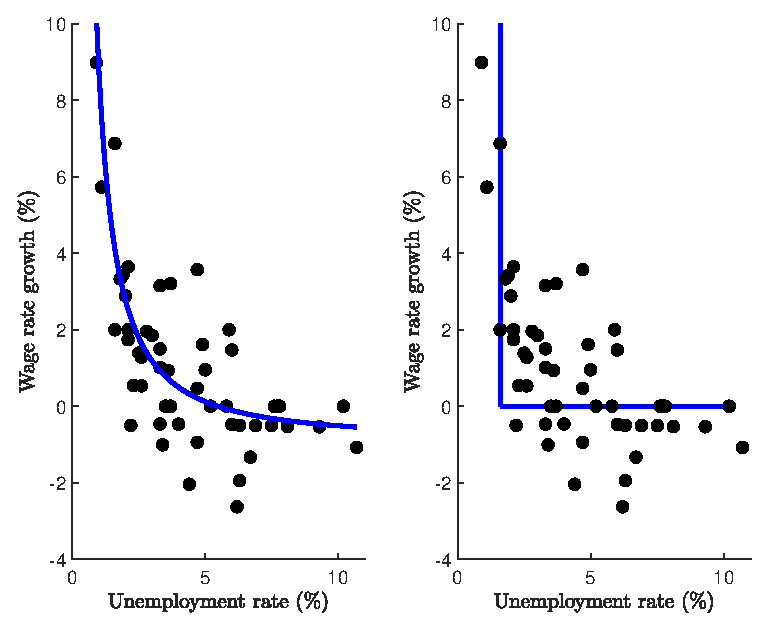
\includegraphics[height=0.80\textheight,keepaspectratio]{Figures/Figure25.eps}

{\scriptsize Left panel: \textcite{Phillips1958}. Right panel: illustrative L-curve.}
\end{frame}

% -----------------------------------------------------------
\begin{frame}{\textcite{Phillips1958}: Key Empirical Findings}
\small
\begin{itemize}
  \item Phillips (1958) studies U.K. data (1861--1957) using scatter plots of:
  \begin{itemize}
    \item wage inflation (rate of change of wage rates),
    \item the unemployment rate.
  \end{itemize}

  \vspace{0.3em}
  \item Core finding for the pre-WWI sample (1861--1913):
  \begin{itemize}
    \item a strong \textbf{negative} relationship between wage inflation and unemployment,
    \item a clear \textbf{non-linearity}: wage inflation rises much faster when unemployment is reduced from already low levels.
  \end{itemize}
\end{itemize}
\end{frame}

% -----------------------------------------------------------
\begin{frame}{\enquote{An Empirical Finding in Search of Theory}}
\small
\begin{itemize}
  \item \textcite{tobin1972} famously described the Phillips curve as \enquote{an empirical finding in search of theory.}
  \item Phillips’ narrative:
  \begin{itemize}
    \item low unemployment leads firms to compete for scarce workers, bidding wages up;
    \item high unemployment makes workers reluctant to accept wages below prevailing rates.
  \end{itemize}
  \item Keynes challenged the orthodox Great Depression interpretation:
  \begin{itemize}
    \item observed wage stickiness does not imply voluntary unemployment;
    \item workers accept lower \textbf{real} wages via higher prices more readily than nominal wage cuts;
    \item nominal wages behave as \enquote{administered prices} (posted and fixed for periods);
    \item workers care about their \textbf{relative} wage across firms.
  \end{itemize}
\end{itemize}
\end{frame}

% -----------------------------------------------------------
\begin{frame}{From Phillips to the Natural Rate of Unemployment}
\small
\begin{itemize}
  \item A literal Phillips reading suggests no unique \enquote{full-employment} anchor—rather, a menu of inflation/unemployment pairs.
  \item The immediate classical objection: wage/price inflation cannot permanently affect unemployment.
  \item \textcite{friedman1969optimum} and \textcite{Phelps1968}:
  \begin{itemize}
    \item confine the inflation--unemployment trade-off to the \textbf{short run};
    \item introduce \textbf{inflation expectations};
    \item define a \textbf{natural rate of unemployment}, determined by labor-market fundamentals and invariant to monetary policy in the long run.
  \end{itemize}
  \item In the 1970s, adverse supply shocks (e.g.\ energy/oil) shifted the curve and complicated identification.
\end{itemize}
\end{frame}



\begin{frame}{Great Inflation: Inflation vs. Unemployment}
\centering
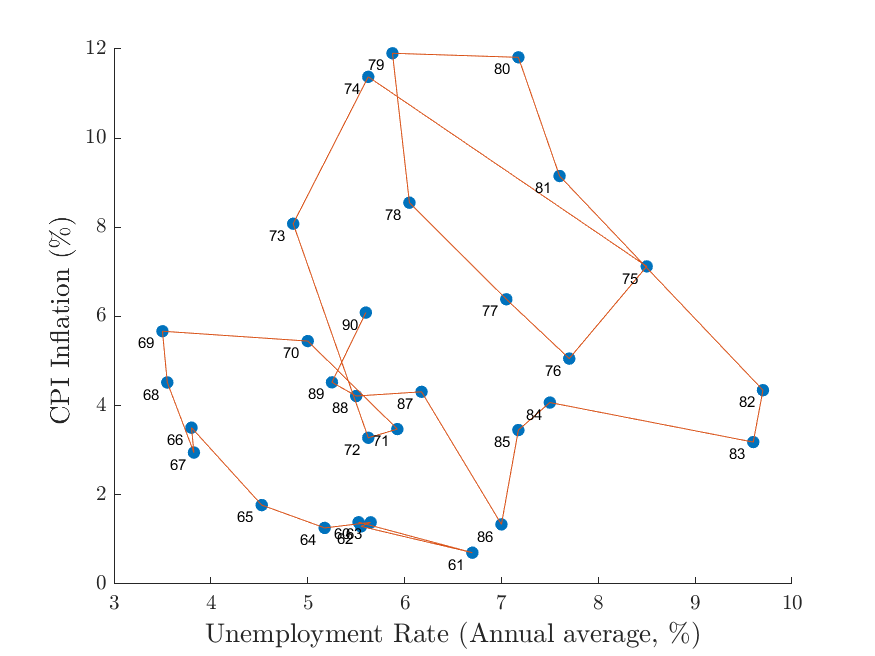
\includegraphics[height=0.82\textheight, keepaspectratio]{Figures/Figure2L.png}
\end{frame}

% -----------------------------------------------------------
\begin{frame}{NK Revival and the Return of Capacity Constraints}
\small
\begin{itemize}
  \item In the 1990s, New-Keynesian models micro-founded a Phillips curve through price-setting frictions:
  \begin{itemize}
    \item staggered pricing implies forward-looking decisions;
    \item monetary shocks can have more \textbf{persistent} real effects.
  \end{itemize}
  \item But the debate shifted away from Keynes’ original emphasis:
  \begin{itemize}
    \item Keynes did not reject full employment; he recast it as a \textbf{capacity ceiling} (maximum aggregate supply);
    \item an \enquote{L-shaped} view: in slack times, demand raises activity with little inflation, whereas in tight markets demand becomes inflationary.
  \end{itemize}
  \item Connection to Friedman’s \textbf{plucking model}: expansions rarely exceed the ceiling, while contractions \enquote{pluck} output below it.
\end{itemize}
\end{frame}
%===========================================================
\section{Outline of the Results}

\begin{frame}{Outline of the Chapter}
\small
\begin{itemize}
  \item Derive the \textbf{natural rate of unemployment} and show why it is independent of monetary policy in the long run.
  \item Introduce \textbf{downward nominal wage rigidity}: in slack markets unemployment becomes demand-determined, while tight markets revert to the natural-rate outcome.
  \item Show how information frictions (delayed information / preset wages) generate a \textbf{short-run} Phillips curve in the spirit of Friedman--Phelps.
  \item Present the \textbf{New-Keynesian Phillips curve (NKPC)} and explain why forward-looking price setting implies \textbf{persistent} monetary non-neutralities.
  \item Combine wage rigidity with the NKPC to obtain an \textbf{L-shaped New-Keynesian Phillips curve} that reconciles flat-slack and steep-tight regimes.
\end{itemize}
\end{frame}
%===========================================================
\section{Natural Rate of Unemployment}
\label{UN}
%===========================================================

\begin{frame}{Households: Heterogeneous Members and Labor Disutility}
\begin{itemize}
  \item We adopt a model of the labor market similar to \textcite{Gali2009}. 
  \item Large number of identical households.
  \item Each household has a continuum of members indexed by $(i,z)\in[0,1]\times[0,1]$:
  \begin{itemize}
    \item $i$: labor type (or age/cohort),
    \item $z$: disutility parameter; if the household is working, disutility is $z^\eta$ with $\eta\ge 0$, otherwise $0$.
  \end{itemize}
\end{itemize}
\textbf{Per-period utility:}
\begin{align*}
U_t
&=\ln C_t-\int_0^1\left(\int_0^{L_t(i)} z^\eta\,dz\right)di
=\ln C_t-\int_0^1\frac{(L_t(i))^{1+\eta}}{1+\eta}\,di,
\end{align*}
where $L_t(i)\in[0,1]$ is the employment fraction of type $i$.
\end{frame}

\begin{frame}{Intertemporal Utility and Consumption Aggregator}
\textbf{Households maximize:}
\begin{equation}
E_{t_0}\left\{ \sum_{t=t_{0}}^{\infty }\beta ^{t-t_{0}}\left[ \ln
C_{t}-\int_{0}^{1}\frac{(L_{t}(i))^{1+\eta }}{1+\eta }di\right] \right\},
\label{eq1}
\end{equation}
with rate of time preferences $0<\beta<1$.
\begin{itemize}
    \item Consumption is a Dixit--Stiglitz aggregator of a continuum of consumption goods $C_t=\left[\int_0^1 C_t(j)^{\frac{\theta-1}{\theta}}\,dj\right]^{\frac{\theta}{\theta-1}}$ where $\theta>1$ is the elasticity of substitution between goods $C(j)$ with $j \in [0,1]$. 
    \item Households optimize with respect to their consumption, saving plans. We assume they have access to an ample spectrum of assets to trade in and that financial markets are complete. 
\end{itemize}
\end{frame}

\begin{frame}{Flow Budget Constraint}
\textbf{Flow budget constraint:}
\begin{equation}
B_{t}+P_{t}C_{t}=\mathcal{W}_{t}+\int_{0}^{1}W_{t}(i)L_{t}(i)di+\Psi
_{t}+\Psi _{t}^{w}-T_{t}.  
\label{eq2}
\end{equation}
\begin{itemize}
    \item $B_t$ is the value of a portfolio with next-period state-contingent payoff $\mathcal{W}_{t+1}$ such that $B_t = E_t(\tilde{R}_{t,t+1}\mathcal{W}_{t+1})$ and nominal discount factor $\tilde{R}_{t,t+1}$ defined in Chapter~5.
    \item Right-hand side represents resources held a time $t$: The payoff of their portfolio $\mathcal{W}_{t+1}$, income $W_t(i)L_t(i)$ for each cohort of workers $i$ and nominal wage $W(i)$, firm profits $\Psi$ less taxes $T$ and profits of the workers' unions $\Psi^w$.
    \item Left-hand side represents spending: Households purchase consumption goods $C_t$ at price $P_t$ and the portfolio of value $B_t$. 
    \item The houeshold problem yields a standard intertemporal budget constraint as in Chapter~5.
\end{itemize}
\end{frame}

\begin{frame}{Euler Equation}
\textbf{First-order conditions:}
\begin{align*}
    \frac{1}{P_t C_t}=\frac{\beta}{\tilde{R}_{t,t+1}}\frac{1}{P_{t+1}C_{t+1}}.
\end{align*}
\begin{itemize}
    \item The above equation characterizes optimal consumption/saving choices at each point in time $t$.
    \item Looking forward from time $t$, there is a set of first-order conditions (Euler equations) equal to the number of states of nature at time $t+1$. 
    \item Optimality implies that the intertemporal budget constraint of the consumers holds with equality. 
\end{itemize}
\end{frame}

% -----------------------------------------------------------
\begin{frame}{Firms: Technology}
\small
\begin{itemize}
  \item Continuum of firms \(j\in[0,1]\) with decreasing returns to labor:
  \[
    Y_t(j)=A_t\big(L_t(j)\big)^{\alpha_L},
    \qquad 0<\alpha_L\le 1,
  \]
  where \(A_t\) denotes technology.
  \item Each firm hires a composite labor input \(L_t(j)\) built from differentiated labor types \(i\in[0,1]\).
\end{itemize}
\end{frame}

% -----------------------------------------------------------
\begin{frame}{Firms: Labor Aggregation and Wage Index}
\small
\begin{itemize}
  \item Firm-level labor aggregator across types \(i\) with elasticity \(\theta_w>1\):
  \[
  L_t(j)=\left(\int_0^1 \big(L_t(i)\big)^{\frac{\theta_w-1}{\theta_w}}\,di\right)^{\frac{\theta_w}{\theta_w-1}}.
  \]
  \item Given nominal wages \(W_t(i)\), define the aggregate wage index:
  \[
  W_t=\left(\int_0^1 \big(W_t(i)\big)^{1-\theta_w}\,di\right)^{\frac{1}{1-\theta_w}}.
  \]
\end{itemize}
\end{frame}

% -----------------------------------------------------------
\begin{frame}{Firms: Demand and Profits}
\small
\begin{itemize}
  \item Demand for firm \(j\) (as in Chapter~5) with \(\theta>1\):
  \[
    Y_t(j)=\left(\frac{P_t(j)}{P_t}\right)^{-\theta}Y_t .
  \]
  \item Profits (with revenue tax \(\tau_t\)):
  \[
    \Psi_t(j)=(1-\tau_t)\,P_t(j)Y_t(j)-W_t\,L_t(j).
  \]
  \item Intuition: profits rise with demand \(Y_t(j)\) and fall with the wage bill \(W_tL_t(j)\).
\end{itemize}
\end{frame}

% -----------------------------------------------------------
\begin{frame}{Price Setting and Labor Demand}
\small
\begin{itemize}
  \item As in Chapter~5, optimal price setting implies a constant markup over marginal cost:
  \[
  \mu_t \equiv \frac{\theta}{(\theta-1)(1-\tau_t)\alpha_L},
  \qquad
  P_t(j)=\mu_t\frac{W_t}{A_t}\big(L_t(j)\big)^{1-\alpha_L}.
  \]
  \item In a symmetric equilibrium, \(P_t(j)=P_t\) and \(L_t(j)=L_t\).
\end{itemize}

\vspace{0.2cm}
\textbf{Aggregate labor demand:}
\begin{equation}
L_{t}=\left( \frac{\mu _{t}}{A_{t}}\frac{W_{t}}{P_{t}}\right) ^{\frac{1}{\alpha _{L}-1}}.
\label{eq3}
\end{equation}
\begin{itemize}
  \item Labor demand is decreasing in the real wage \(W_t/P_t\) since \(\alpha_L-1<0\).
\end{itemize}

\vspace{0.2cm}
\textbf{Labor demand for type \(i\):}
\begin{equation}
L_{t}(i)=\left( \frac{W_{t}(i)}{W_{t}}\right) ^{-\theta _{w}}L_{t}.
\label{eq4}
\end{equation}
\end{frame}

\begin{frame}{Unions: Objective and Optimal Wage Setting}
\begin{itemize}
    \item Union for type $i$ chooses $W_t(i)$ taking demand \eqref{eq4} as given.
\end{itemize}
\textbf{Objective function:}
\begin{equation}
\Psi _{t}^{w}=\lambda _{t}W_{t}(i)L_{t}(i)-\frac{L_{t}(i)^{1+\eta }}{1+\eta },
\label{eq5}
\end{equation}
where $\lambda_t=\frac{1}{P_t C_t}$ converts nominal income into marginal utility units. \\
\vspace{1em}
\textbf{First-order condition (monopoly wage setting):}
\[
\frac{W_t(i)}{P_t}=\mu^w\,C_t\,L_t(i)^\eta.
\]
with markup $\mu^w\equiv \frac{\theta_w}{\theta_w-1}.$
\end{frame}

\begin{frame}{Natural Employment Rate}
\small
\begin{itemize}
    \item In a symmetric equilibrium, \(W_t(i)=W_t\) and \(L_t(i)=L_t\) for all \(i\).
\end{itemize}

This implies the \textbf{labor-supply} relation:
\begin{equation}
L_{t}=\left( \frac{1}{\mu ^{w}}\frac{W_{t}}{P_{t}C_{t}}\right) ^{\frac{1}{\eta }}.
\label{eq6}
\end{equation}

The intersection between labor demand \eqref{eq3} and labor supply \eqref{eq6} yields the \textbf{natural rate of employment}:
\[
L_t^n=\left(\frac{1}{\mu^w}\frac{1}{\mu_t}\right)^{\frac{1}{1+\eta}}.
\]

\begin{itemize}
    \item In the flexible-wage equilibrium, the real wage adjusts so that employment equals \(L_t^n\).
    \item Natural employment \(L_t^n\) depends only on goods-market and labor-market markups \((\mu_t,\mu^w)\).
    \item It does not depend on demand conditions or inflation.
\end{itemize}
\end{frame}

\begin{frame}{Unemployment Rate (following \textcite{Gali2009})}
\small
\begin{itemize}
    \item A type-\(i\) worker supplies labor iff the real wage covers disutility:
    \[
      \frac{W_t(i)}{P_t}\ge C_t z^{\eta}.
    \]
    \item The marginal worker defines labor-force participation \(L_t^{s}(i)\):
    \[
      \frac{W_t(i)}{P_t} = C_t\big(L_t^{s}(i)\big)^{\eta}.
    \]
    \item In symmetry, \(W_t(i)=W_t\) and \(L_t^{s}(i)=L_t^{s}\), so
    \begin{align}
        L_{t}^{s}=\left( \frac{W_{t}}{P_{t}C_{t}}\right) ^{\frac{1}{\eta }}.
        \label{eq7}
    \end{align}
    \item Comparing \eqref{eq7} with \eqref{eq6} yields the \textbf{natural unemployment rate}:
    \begin{align}
        u^{n}\equiv 1-\frac{L_{t}^{n}}{L_{t}^{s}}
        =1-\left( \frac{1}{\mu ^{w}}\right)^{\frac{1}{\eta }}.
        \label{eq8}
    \end{align}
\end{itemize}
\end{frame}

\begin{frame}{Equilibrium Employment}
\label{Slide25}
\small
\begin{columns}[T,totalwidth=\textwidth]

% -------- Left column: figure --------
\begin{column}{0.52\textwidth}
\centering
\vspace{-0.2cm}

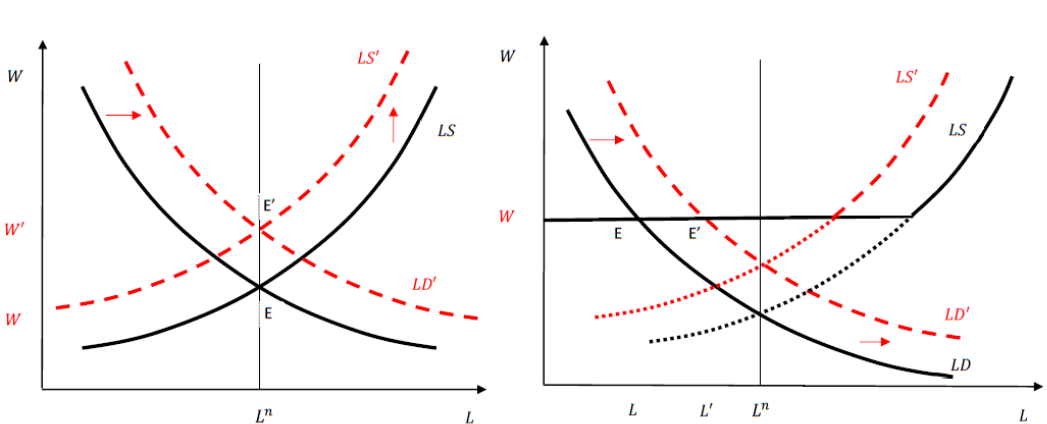
\includegraphics[trim=0 0 12.8cm 0, clip, width=\linewidth]{Figures/Figure26.png}
{\scriptsize
An increase in the price level \(P_t\) shifts both \(LD\) and \(LS\) upward to \(LD'\) and \(LS'\), raising the nominal wage while leaving employment at \(L^n\).
}
\end{column}

% -------- Right column: explanation --------
\begin{column}{0.42\textwidth}
\begin{itemize}
  \item Labor supply and demand are plotted in \textbf{nominal wage--employment} space.
  \item A proportional increase in \(P_t\) shifts both \(LS\) and \(LD\) upward by the same factor.
  \item \textbf{Result:} employment remains at the natural level \(L^n\); only the nominal wage scales up.
  \item Hence, with flexible prices and wages, unemployment is \textbf{independent} of inflation.
\end{itemize}
\end{column}

\end{columns}
\end{frame}
%===========================================================
\section{Keynesian Unemployment}
\label{SectionKU}
%===========================================================

\begin{frame}{Keynesian Unemployment via Downward Nominal Wage Rigidity}
\begin{itemize}
    \item Assume nominal wages cannot fall below a lower bound \textcolor{red}{$W$}. 
    \item Unions again maximize \eqref{eq5} under demand \eqref{eq4} but with the constraint 
\[
W_t(i)=\max\left\{\textcolor{red}{W},\ \mu^w C_t L_t(i)^\eta \right\}.
\]    \item This again implies symmetry across different cohorts $W_t(i)=W_t$ and $L_t(i)=L_t$.
    \item Implications for labor supply: 
    \begin{itemize}
        \item If the labor market is slack: $W_t=\textcolor{red}{W}$ binds and labor supply is perfectly elastic at \textcolor{red}{W}.
        \item If the labor market is tight: $W_t>\textcolor{red}{W}$ implying a return to the flexible-wage upward-sloping schedule.
    \end{itemize}
\end{itemize}
\end{frame}



\begin{frame}{Labor Demand in Terms of Nominal Spending}
\begin{itemize}
    \item By using $Y_t = A_tL_t^{\alpha_L}$ and defining nominal spending as $\tilde{Y} = P_tY_t$ we can rewrite labor demand \eqref{eq3}: 
    \begin{align*}
        L_t=\frac{1}{W_t}\frac{\tilde{Y}_t}{\mu_t}.
    \end{align*}
    \item When the wage floor binds ($W_t=\textcolor{red}{W}$), employment becomes:
\[
L_t=\frac{1}{\textcolor{red}{W}}\frac{\tilde{Y}_t}{\mu_t}.
\]
    \item This shows that higher nominal spending can directly boost employment in slack markets. 
\end{itemize}
\end{frame}

\begin{frame}{Unemployment at the Wage Floor}
\begin{itemize}
    \item When $W_t = \textcolor{red}{W}$ and using $P_tC_t=P_tY_t = \tilde{Y}_t$, labor force is given by: 
    \begin{align*}
        L_t^s=\left(\frac{\textcolor{red}{W}}{\tilde{Y}_t}\right)^{\frac{1}{\eta}}
    \end{align*}
    \item Recall that employment is $L_t = \frac{1}{\textcolor{red}{W}}\frac{\tilde{Y}}{\mu_t}$, unemployment rate is then given by: 
    \begin{align*}
        u_t=1-\frac{L_t}{L_t^s}
=1-\frac{1}{\mu_t}\left(\frac{\tilde{Y}_t}{\textcolor{red}{W}}\right)^{1+\frac{1}{\eta}}.
    \end{align*}
    \begin{itemize}
        \item $u_t$ decreases in nominal spending $\tilde{Y}_t$ and increases in the markup $\mu_t$.
        \item Policy that increases nominal spending $\tilde{Y}_t$ reduced unemployment, when labor market is slack.
    \end{itemize}
\end{itemize}
\end{frame}

\begin{frame}{Threshold Nominal Spending}
\begin{itemize}
    \item Define $\tilde{Y}_t^\ast$ as the nominal spending level at which the flexible wage exceeds the norm $\textcolor{red}{W}$. The threshold is:
    \begin{align*}
        \tilde{Y}_{t}^{\ast }=\frac{\textcolor{red}{W}}{\mu _{t}}\left( \frac{1}{\mu ^{w}\mu _{t}}\right) ^{\frac{\eta }{1+\eta }}.
    \end{align*}
  \item If $\tilde{Y}_t<\tilde{Y}_t^\ast$: wage floor binds, level of unemployment is driven by insufficient aggregate demand. 
  \item If $\tilde{Y}_t\ge\tilde{Y}_t^\ast$: $W_t>\textcolor{red}{W}$, economy returns to the flexible-wage outcome:
  \[
  L_t=L_t^n=\left(\frac{1}{\mu^w\mu_t}\right)^{\frac{1}{1+\eta}},
  \]
  with unemployment at the natural rate \eqref{eq8}.
\end{itemize}
\end{frame}

\begin{frame}{Equilibrium Employment}
\label{Slide31}
\small
\begin{columns}[T,totalwidth=\textwidth]

% -------- Left column: figure --------
\begin{column}{0.58\textwidth}
\centering
\vspace{-0.2cm}

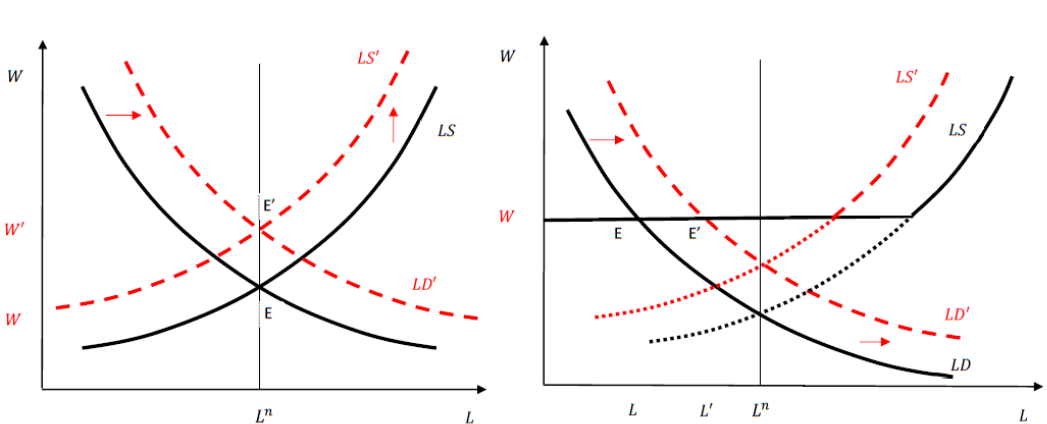
\includegraphics[trim=11.3cm 0 0 0, clip, width=\linewidth]{Figures/Figure26.png}
\end{column}

% -------- Right column: interpretation --------
\begin{column}{0.42\textwidth}
\begin{itemize}
    \item Wage floor: \(W_t=\textcolor{red}{W}\). If \(\tilde Y_t<\tilde Y_t^\ast\), the constraint binds and employment is demand-determined.
    \item Initial equilibrium \(E\): \(L<L^n\) and \(u>u^n\).
    \item Higher nominal spending shifts \(LD\to LD'\) (and \(LS\to LS'\)), moving the economy to \(E'\).
    \item Result: \(L\uparrow\) and \(u\downarrow\). Nominal spending reduces unemployment.
\end{itemize}
\end{column}

\end{columns}
\end{frame}
\begin{frame}{Asymmetry and the Plucking Interpretation}
\small
\begin{itemize}
  \item \textbf{Keynesian asymmetry:}
  \begin{itemize}
    \item \textbf{Slack is common:} when unemployment is above its natural rate, higher aggregate demand can raise \(L_t\) with limited inflation pressure.
    \item \textbf{Tightness is exceptional:} near full employment, capacity constraints bind and additional demand translates mainly into inflation rather than higher employment.
  \end{itemize}

  \vspace{0.4em}
  \item \textbf{Friedman’s plucking model} \parencite{friedman1964} mirrors this logic:
  \begin{itemize}
    \item output typically fluctuates near a \textbf{ceiling} (capacity),
    \item recessions \enquote{pluck} the economy below the ceiling; recoveries largely reflect the return toward it.
  \end{itemize}

  \vspace{0.4em}
  \item \textbf{Policy emphasis differs:}
  \begin{itemize}
    \item Friedman highlights monetary policy as the key tool to stabilize contractions and limit deep \enquote{plucks}.
    \item Keynes places greater weight on fiscal policy.
  \end{itemize}
\end{itemize}
\end{frame}
%===========================================================
\section{Short-Run Non-Neutralities}
\label{SR}
%===========================================================

\begin{frame}{Departure from the Natural Rate}
\begin{itemize}
    \item Historically, the key departure from the ideal neoclassical world is the acknowledgment of information frictions leading to imperfect price adjustments. 
    \vspace{1em}
    \item We consider the framework detailed in Section~\ref{UN} and the optimization problem faced by unions under information frictions. 
    \vspace{1em}
    \item We assume that unions do not have updated information on the state of the economy: one-period delayed information. 
\end{itemize}
\end{frame}

\begin{frame}{Information Frictions: Wage Setting with $t\!-\!1$ Information}
\begin{itemize}
    \item Unions maximize~\eqref{eq5} with information from the previous period $t-1$, which implies the wage $$W_t=\mu^w\,E_{t-1}\{P_t Y_t L_t^\eta\}$$ in a symmetric equilibrium. 
    \item Labor demand is unchanged: 
    \begin{align}
        L_{t}=\frac{1}{\mu _{t}}\frac{P_{t}Y_{t}}{W_{t}}. 
        \label{eq9}
    \end{align}
    \item ...but wages are set with the previous-period information.
    \item This framework generates a short-run Phillips curve relation around the natural rate.
\end{itemize}
\end{frame}

\begin{frame}{Log-Linearization: Wage and Labor Equations}
\begin{itemize}
    \item A first order approximation around the non-stochastic steady state of the two above equations: 
    \begin{align}
        \hat{W}_{t}=E_{t-1}\left\{ \hat{P}_{t}+\eta \hat{L}_{t}+\hat{Y}_{t}\right\}, \label{eq10}\\
        \hat{L}_{t}=\hat{P}_{t}+\hat{Y}_{t}-\hat{W}_{t}-\hat{\mu}_{t}. \label{eq11}
    \end{align}
    in which a variable with a hat denotes log-deviations with respect to the steady state. 
    \item Take $E_{t-1}$ of \eqref{eq11} and substitute into \eqref{eq10}: $$E_{t-1}\hat{L}_{t}=-\frac{E_{t-1}\{\hat{\mu}_t\}}{1+\eta}$$ and therefore $E_{t-1}\hat{L}_{t}=E_{t-1}\hat{L}_t^n$.
\end{itemize}
\end{frame}

% --- Slide 1 ---
\begin{frame}{Expectations-Augmented Phillips Curve}
\small
\begin{itemize}
    \item Combining \eqref{eq10} and \eqref{eq11} yields deviations of employment from the expected natural level:
    \[
    \hat{L}_{t}-E_{t-1}\hat{L}_{t}^{n}
    =(\hat{P}_{t}+\hat{Y}_{t})-E_{t-1}(\hat{P}_{t}+\hat{Y}_{t})
    -(\hat{\mu}_{t}-E_{t-1}\hat{\mu}_{t}).
    \]
    \item \textbf{Interpretation:}
    \begin{itemize}
        \item Unexpected movements in nominal spending \((\hat{P}_{t}+\hat{Y}_{t})-E_{t-1}(\hat{P}_{t}+\hat{Y}_{t})\) raise employment relative to its expected natural level.
        \item Unexpected increases in markups \((\hat{\mu}_{t}-E_{t-1}\hat{\mu}_{t})\) reduce employment relative to its expected natural level.
        \item The effects are symmetric: positive and negative surprises move employment in opposite directions.
    \end{itemize}
\end{itemize}
\end{frame}

% --- Slide 2 ---
\begin{frame}{Expectations-Augmented Phillips Curve}
\small
\begin{itemize}
    \item Using \(\hat L_t=\alpha_L^{-1}(\hat Y_t-\hat A_t)\), we obtain the expectations-augmented Phillips curve:
    \begin{align}
        \pi _{t}=E_{t-1}\pi _{t}+k(\hat{Y}_{t}-\hat{Y}_{t}^{n})+\upsilon _{t},
        \label{eq12}
    \end{align}
    where \(\pi_t=\hat P_t-\hat P_{t-1}=p_t-p_{t-1}\) and \(k\equiv \frac{1-\alpha_L}{\alpha_L}\).
    
    \vspace{0.3cm}
    \item The composite shock term is
    \[
    \upsilon_t
    =\frac{\eta +\alpha _{L}}{1+\eta }(\hat{\mu}_{t}-E_{t-1}\hat{\mu}_{t})
    -(\hat{A}_{t}-E_{t-1}\hat{A}_{t}),
    \]
    and the (log) natural output is
    \[
    \hat{Y}_{t}^{n}\equiv \hat{A}_{t}-\frac{\alpha _{L}}{1+\eta }\hat{\mu}_{t}.
    \]
\end{itemize}
\end{frame}
\begin{frame}{Phillips Curve with Unemployment}
\begin{itemize}
    \item Combine \eqref{eq7} and \eqref{eq9} to obtain $$\frac{L_t}{L_t^s}=\mu_t^{\frac{1}{\eta}}L_t^{ 1+\frac{1}{\eta}}.$$
    \item Using $u_t=1-\frac{L_t}{L_t^s}$ and the approximation $u_t \approx -\ln(L_t/L_t^s)$ for small $u$: $$u_t-u^n= -\left(1+\frac{1}{\eta}\right)(\hat L_t-\hat L_t^n)$$. 
    \item Therefore, \eqref{eq12} can be written as: 
    \begin{align}
        \pi _{t}=E_{t-1}\pi _{t}-k_{u}(u_{t}-u^{n})+\upsilon _{t}, 
        \label{eq13}
    \end{align}
    with $k_u=\frac{(1-\alpha_L)\eta}{1+\eta}.$
\end{itemize}
\end{frame}

\begin{frame}{Key Features of the Expectations-Augmented Phillips Curve}
\small
\begin{itemize}
    \item \textbf{Common foundations:} Output-gap and unemployment formulations measure slack differently, but share the same structure and policy implications for the inflation--activity trade-off.

    \item \textbf{Short-run non-neutrality:} Monetary disturbances have transitory real effects. Under rational expectations, adjustment can occur quickly (even within one period).

    \item \textbf{Only surprises matter:} Systematic policy cannot permanently raise real activity. Only unexpected inflation can move output or unemployment away from natural levels.

    \item \textbf{Symmetry around the natural rate:} Positive and negative deviations from the natural rate generate symmetric inflationary or disinflationary pressures.

    \item \textbf{Inflation is not pinned down:} The model does not uniquely determine the inflation rate. Real variables return to natural levels once expectations align with outcomes, not necessarily with the target.
\end{itemize}
\end{frame}

\begin{frame}{Great Inflation: Inflation vs. Unemployment}
\centering
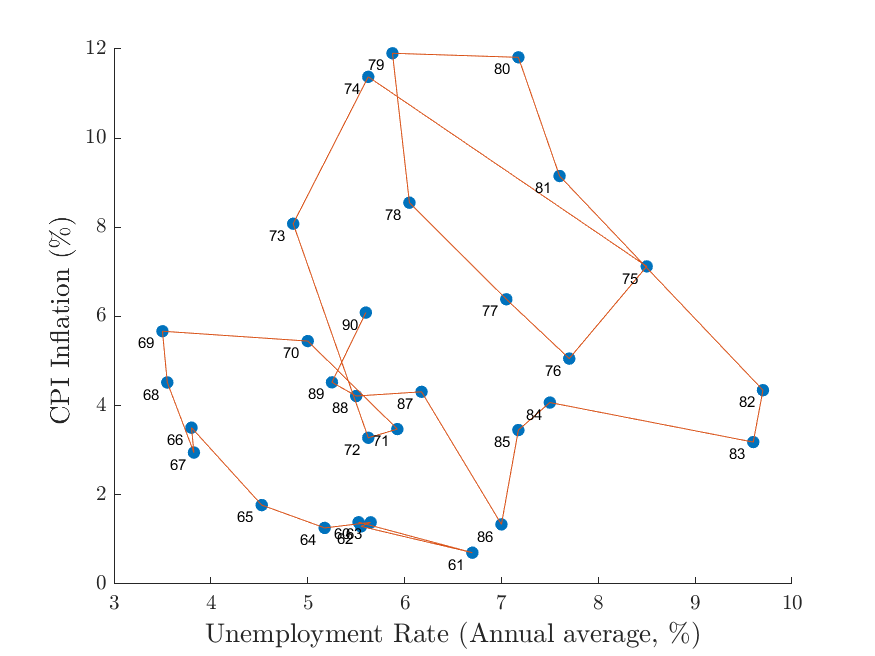
\includegraphics[height=0.82\textheight, keepaspectratio]{Figures/Figure2L.png}
\end{frame}

% -----------------------------------------------------------
\begin{frame}{Inflation and Unemployment in the US (Time Series)}
\label{InflUnemplFigures}
\centering
\vspace{-0.2cm}
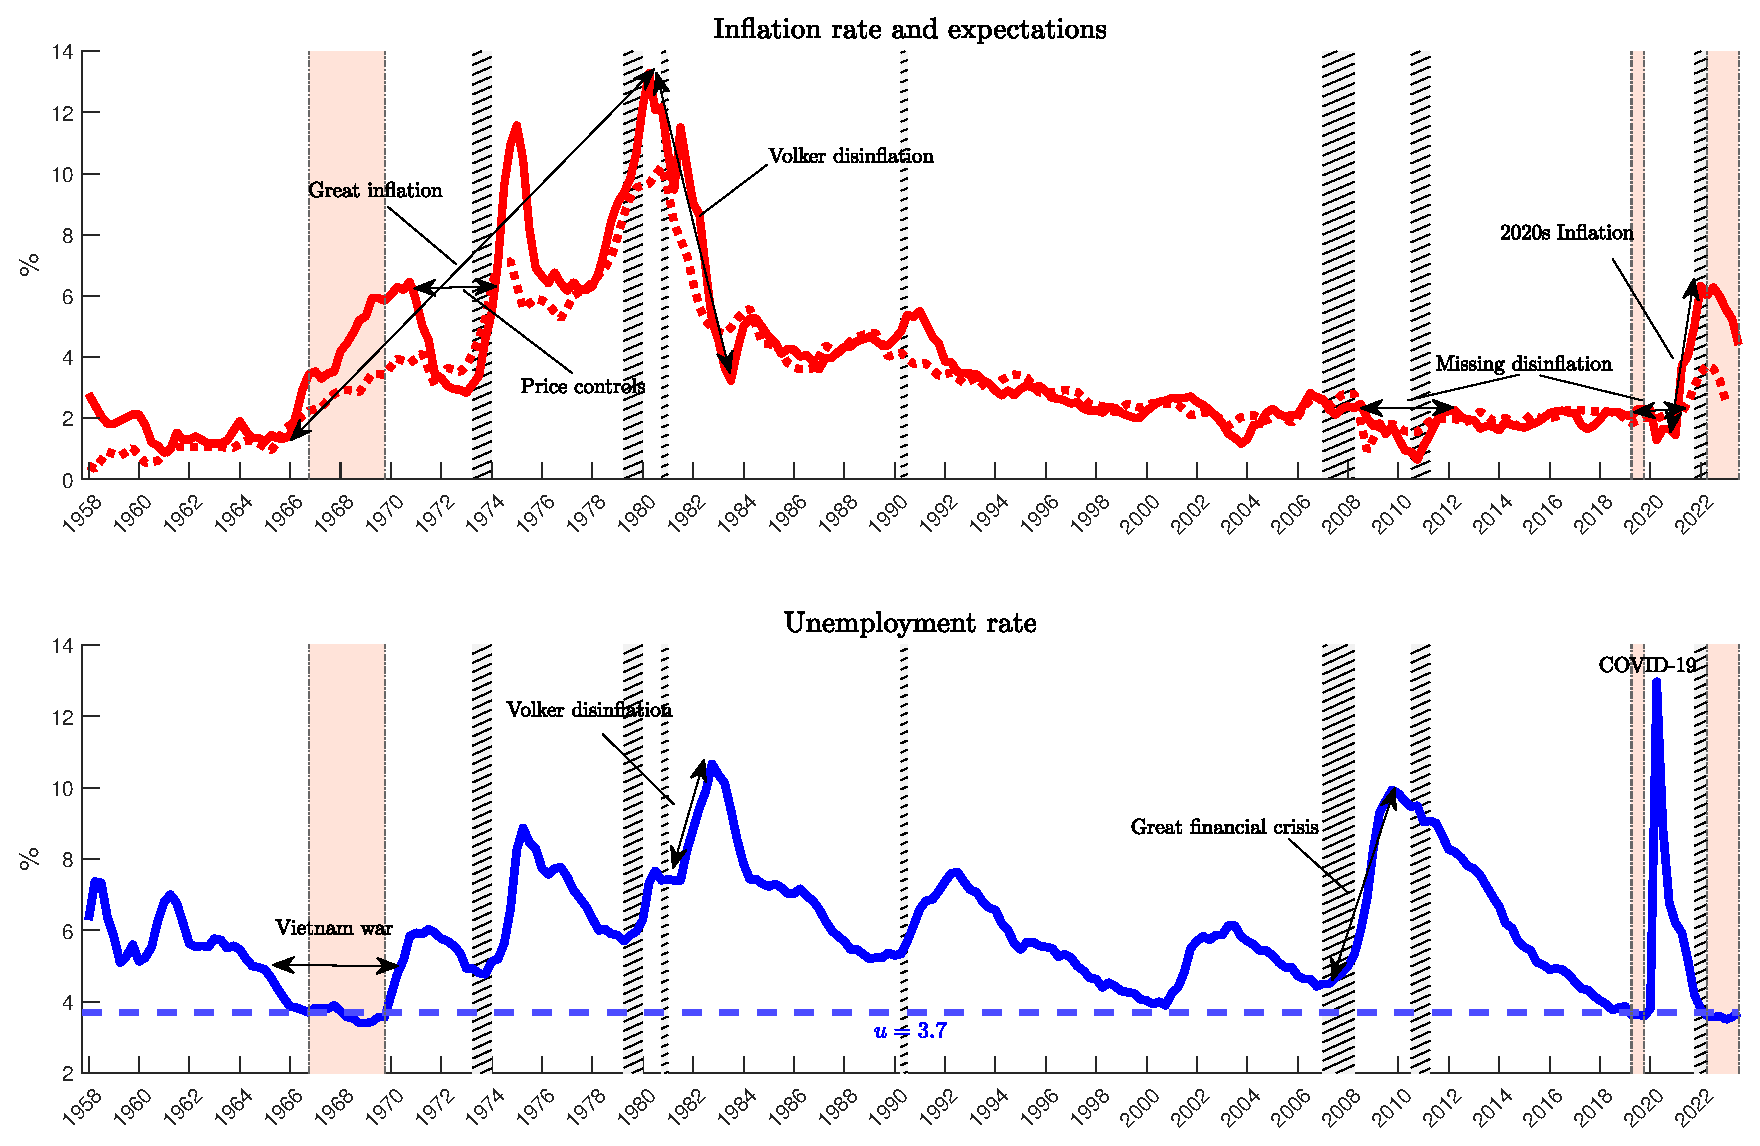
\includegraphics[height=0.65\textheight,keepaspectratio]{Figures/Figure24.eps}

\vspace{0.3cm}
\small
\begin{itemize}
  \item Evolution of U.S. inflation and inflation expectations (top panel) and the unemployment rate (bottom panel).
\end{itemize}
\end{frame}


\begin{frame}{Great Inflation through the Phillips Curve Lens}
\small
\begin{itemize}
    \item In the mid-1960s, inflation rose while unemployment was low, seemingly consistent with a short-run Phillips-curve trade-off.

    \item Monetary tightening in the late 1960s reduced output and raised unemployment—movement along the short-run curve.

    \item Over time, inflation expectations drifted upward, shifting the Phillips curve and weakening the apparent trade-off.

    \item Policy easing, wage and price controls, and adverse supply shocks contributed to stagflation: high inflation alongside high unemployment.

    \item The expectations-augmented Phillips curve explains why higher expected inflation translates into higher actual inflation at a given unemployment rate.

    \item The Volcker disinflation reduced inflation by tightening policy and lowering inflation expectations—at the cost of a sharp rise in unemployment.
\end{itemize}
\end{frame}
%===========================================================
\section{Persistent Monetary Non-Neutralities}
\label{PN}
%===========================================================

% -----------------------------------------------------------
\begin{frame}{Persistent Monetary Non-Neutralities}
\small
\begin{itemize}
    \item The expectations-augmented Phillips curve limits the inflation--output trade-off to the short run.
    \item Inflation expectations anchor the economy around the natural rate of output (or unemployment).
    \item Under rational expectations, one-time increases in nominal spending have only transitory real effects.
    \item Empirically, monetary shocks often generate hump-shaped responses in real activity.
    \item New-Keynesian models explain persistence through nominal rigidities and staggered price setting.
\end{itemize}
\end{frame}

% -----------------------------------------------------------
\begin{frame}{New-Keynesian Phillips Curve (NKPC)}
\small
\textbf{The benchmark NKPC} (from Chapter~5):
\begin{align}
   \pi _{t}-\pi
   =\kappa (\hat{Y}_{t}-\hat{Y}_{t}^{n})
   +\beta E_{t}(\pi_{t+1}-\pi ).
\label{eq14} 
\end{align}
\begin{itemize}
  \item The equation is similar to \eqref{eq12}, but it features forward-looking inflation expectations \(E_t(\pi_{t+1}-\pi)\) rather than past-period expectations of current inflation.
  \item This reflects the forward-looking behavior of price setters under Calvo pricing.
  \item As a result, monetary shocks can have persistent effects on output and inflation.
  \item Keeping inflation on target requires the entire expected path of output gaps to be zero, not only the current gap.
\end{itemize}
\end{frame}

% -----------------------------------------------------------
\begin{frame}{Nominal Spending and the Price-Level Phillips Curve}
\small
\textbf{Log nominal spending} follows:
\begin{align}
    \tilde{y}_{t}=\pi +\tilde{y}_{t-1}+\varepsilon _{t}.
    \label{eq15}
\end{align}
\begin{itemize}
    \item \(\varepsilon_t\) is white noise, \(\pi\) is the inflation target, and \(\tilde y_t=p_t+y_t\).
    \item The NKPC can be rewritten as:
    \begin{align*}
        p_t-p_{t-1}-\pi=\kappa(\tilde y_t-p_t)+\beta E_t(p_{t+1}-p_t-\pi).
    \end{align*}
    \item This stochastic second-order difference equation can be written using the lag operator \(\mathsf{L}\) (Chapter~7):
    \begin{align*}
        \left[ \mathsf{L}^{-1}-\left( 1+\frac{1}{\beta }+\frac{\kappa }{\beta }\right)
        +\frac{1}{\beta }\mathsf{L}\right] p_{t}
        =-\frac{\kappa }{\beta }\tilde{y}_{t}-\frac{1-\beta }{\beta }\pi.
    \end{align*}
\end{itemize}
\end{frame}

% -----------------------------------------------------------
\begin{frame}{Eigenvalues}
\small
\begin{itemize}
    \item Characterizing the previous equation in terms of eigenvalues \(\gamma_1,\gamma_2\) associated with the characteristic polynomial yields
    \[
    \left[ \mathsf{L}^{-1} - (\gamma_1 + \gamma_2) + \gamma_1 \gamma_2 \mathsf{L} \right] p_t
    = -\gamma_1 \gamma_2 \kappa \tilde{y}_t
    - \gamma_1 \gamma_2 (1 - \beta)\pi,
    \]
    with \(0<\gamma_1<1<\gamma_2\).
    \item The eigenvalues satisfy
    \begin{align}
        \gamma _{1}+\gamma _{2} &=1+\frac{1}{\beta }+\frac{\kappa }{\beta }, 
        \label{eq16} \\
        \gamma _{1}\gamma _{2} &=\frac{1}{\beta }.  \label{eq17}
    \end{align}
    \item Hence
    \[
    (1-\gamma_1\mathsf{L})(1-\gamma_2^{-1}\mathsf{L}^{-1})p_t
    =\gamma_1\kappa \tilde y_t+\gamma_1(1-\beta)\pi.
    \]
\end{itemize}
\end{frame}

% -----------------------------------------------------------
\begin{frame}{Solving for Prices}
\small
\begin{itemize}
    \item Solving the previous equation (as in Chapter~7) gives
    \[
    p_t
    = \gamma_1 p_{t-1}
    + \frac{\kappa}{\beta(\gamma_2 - 1)} \tilde{y}_t
    + \left(
        \frac{\kappa}{\beta(\gamma_2 - 1)^2}
        + \frac{1 - \beta}{\beta(\gamma_2 - 1)}
      \right)\pi .
    \]
    \item Using \eqref{eq16} and \eqref{eq18}, this simplifies to
    \begin{align}
        p_{t}=\gamma _{1}(\pi +p_{t-1})+(1-\gamma _{1})\tilde{y}_{t}.
        \label{eq18}
    \end{align}
    \item Equivalently, using \eqref{eq15}:
    \[
    p_t = \pi + \gamma_1 p_{t-1} + (1 - \gamma_1)(\tilde{y}_{t-1} + \varepsilon_t).
    \]
\end{itemize}
\end{frame}

% ---------------------------------------------------

\begin{frame}{Propagation of a Nominal Spending Shock}
\small
\begin{itemize}
    \item A one-time innovation in nominal spending \(\varepsilon_t\) raises prices on impact by \((1-\gamma_1)\varepsilon_t\).
    \item The shock propagates into future prices, decaying geometrically at rate \(\gamma_1\).
    \item Output responds on impact and then returns gradually toward its steady state at rate \(\gamma_1\).
    \item \(\gamma_1\) governs the magnitude and persistence of real effects; it is inversely related to the slope \(\kappa\) of the NK Phillips curve.
    \item \textbf{Contrast with the New Classical Phillips curve:} with frictionless prices, only \emph{unexpected} nominal shocks matter and real effects are much less persistent; NK frictions provide a mechanism for delayed and hump-shaped responses.
    \item Price rigidities and strategic complementarities amplify persistence and improve empirical fit.
\end{itemize}
\end{frame}
%===========================================================
\section{A L-shaped New-Keynesian Phillips Curve}
\label{Inv-L}
%===========================================================

% -----------------------------------------------------------
\begin{frame}{Inflation and Unemployment in the US (Time Series)}
\label{InflUnemplFiguresTS}
\centering
\vspace{-0.2cm}
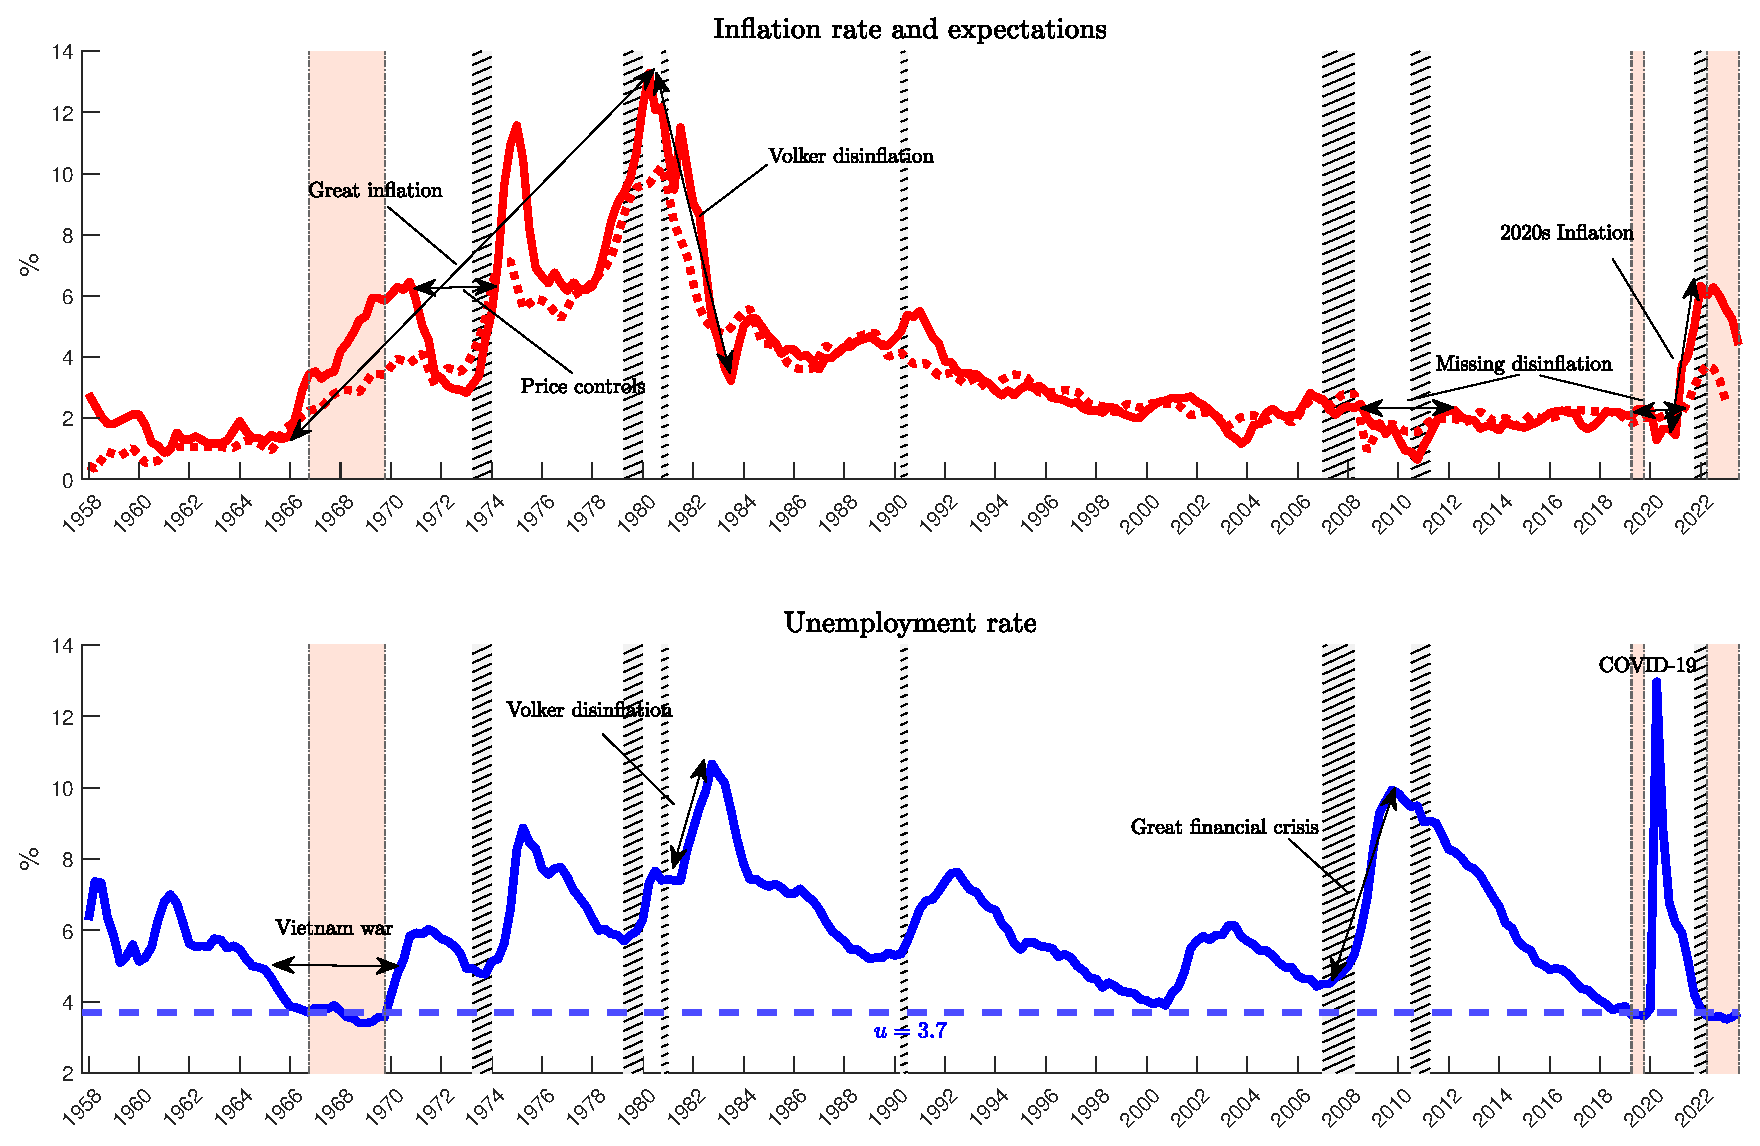
\includegraphics[height=0.60\textheight,keepaspectratio]{Figures/Figure24.eps}

\vspace{0.3cm}
\small
\begin{itemize}
  \item Evolution of U.S. inflation and inflation expectations (top panel) and the unemployment rate (bottom panel).
\end{itemize}
\end{frame}

% -----------------------------------------------------------
\begin{frame}{Inflation and Unemployment in the US (Scatter Plots)}
\label{InflUnemplFiguresSC}
\centering
\vspace{-0.2cm}
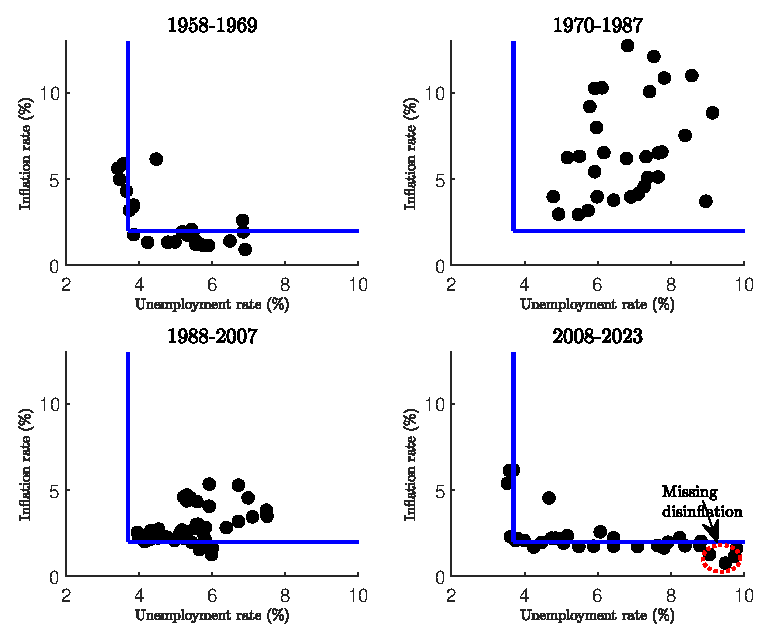
\includegraphics[height=0.78\textheight,keepaspectratio]{Figures/Figure27.eps}

\small
\begin{itemize}
  \item Scatter plots of CPI inflation and the unemployment rate for different U.S. samples.
\end{itemize}
\end{frame}

\begin{frame}{Missing Disinflation and Post-COVID Inflation}
\small
\begin{itemize}
  \item \textbf{Missing disinflation (Great Recession \& COVID):} Slide~\ref{InflUnemplFiguresTS} shows that large unemployment spikes did not generate large disinflations \(\Rightarrow\) a very flat Phillips curve in slack markets.
  \vspace{1em}
  \item \textbf{Post-COVID surge:} Inflation rose sharply once labor markets became unusually tight (Slide~\ref{InflUnemplFiguresTS}) \(\Rightarrow\) a steep/vertical segment near full employment.
  \vspace{1em}
  \item \textbf{Kinked \enquote{L-curve}} \parencite{BenignoEggertsson2023}: scatter evidence in Slide~\ref{InflUnemplFiguresSC}; vertical segment around \(u^{n}\approx 3.7\%\), flat segment around \(\pi \approx 2\%\).
\end{itemize}
\end{frame}

% -----------------------------------------------------------
\begin{frame}{Slack vs.\ Tight Labor Markets}
\small
The model assumes the following \textbf{piecewise wage setting}:
\[
W_{t}=\left\{
\begin{array}{cccc}
W_{t-1}(\Pi _{t}^{e})^{\delta _{\pi }} &  & \text{if} & u_{t}>u^{n} \\
\\
W_{t}^{\mathrm{flex}}=\mu ^{w}P_{t}Y_{t}L_{t}^{\eta } &  & \text{if} & u_{t}=u^{n}
\end{array}
\right.
\]
\begin{itemize}
    \item \textbf{Slack labor market} (\(u_t>u^n\)): wages do not fall below the previous level and adjust to expected inflation \(\Pi_t^e\) via \(\delta_\pi\ge 0\).
    \item \textbf{Tight labor market} (\(u_t=u^n\)): wages follow the flexible-wage outcome (Section~\ref{UN}).
\end{itemize}

\textbf{In log deviations from steady state, real wages are:}
\begin{align}
\hat{w}_{t}=\left\{
\begin{array}{cccc}
\hat{w}_{t-1}-(\pi _{t}-\pi )+\delta _{\pi }E_{t}(\pi _{t+1}-\pi ) &  &
\text{if} & u_{t}>u^{n} \\
\\
\hat{Y}_{t}+\eta \hat{L}_{t} &  & \text{if} & u_{t}=u^{n}
\end{array}
\right. .
\label{eq19}
\end{align}
\end{frame}

% -----------------------------------------------------------
\begin{frame}{NKPC in Terms of Marginal Costs}
\small
\begin{itemize}
    \item The NKPC can be written in terms of real marginal costs:
    \begin{align}
        \pi _{t}-\pi
        =k_{m}(\hat{\mu}_{t}+\hat{w}_{t}+\hat{L}_{t}-\hat{Y}_{t})
        +\beta E_{t}(\pi _{t+1}-\pi ),
        \label{eq20}
    \end{align}
    where \(k_m>0\).

    \item \textbf{Tight labor market} (\(u_t=u^n\)): substitute the second line of \eqref{eq19} into \eqref{eq20} to obtain
    \begin{align}
        \pi _{t}-\pi
        =k_{m}\big[(1+\eta )\hat{L}_{t}+\hat{\mu}_{t}\big]
        +\beta E_{t}(\pi_{t+1}-\pi ),
        \label{eq21}
    \end{align}

    \item \textbf{Slack labor market} (\(u_t>u^n\)): using the first line of \eqref{eq19} yields
    \begin{align}
        \pi _{t}-\pi
        =\tilde{k}_{m}\big[\hat{w}_{t-1}+(1-\alpha _{L})\hat{L}_{t}+\hat{\mu}_{t}-\hat{A}_{t}\big]
        +\tilde{k}_{\pi }E_{t}(\pi _{t+1}-\pi ),
        \label{eq22}
    \end{align}
    with \(\tilde{k}_{m}=\frac{k_{m}}{1+k_{m}}\) and \(\tilde{k}_{\pi }=\frac{\beta +k_{m}\delta _{\pi }}{1+k_{m}}\).
\end{itemize}
\end{frame}

% -----------------------------------------------------------
\begin{frame}{Key Implications}
\small
Key implications of \eqref{eq21} and \eqref{eq22}:
\begin{itemize}
    \item The Phillips curve is flatter in a slack labor market (since \(\tilde{k}_{m}<k_{m}\)).
    \item The response to a markup shock (e.g.\ an energy/oil-price shock) is smaller when the labor market is slack.
    \item Since \eqref{eq22} contains lagged real wages, inflation is more sluggish in slack labor markets.
    \item The sensitivity to inflation expectations, \(\tilde{k}_\pi\), can be larger or smaller than \(\beta\) depending on the degree of wage indexation \(\delta_\pi\).
\end{itemize}
\end{frame}

% -----------------------------------------------------------
\begin{frame}{Implications for Unemployment}
\small
\textbf{Tight labor market (\(u_t=u^n\))}
\begin{itemize}
    \item With flexible wages, unemployment remains at the natural rate.
    \item From \eqref{eq21}, inflation is determined by demand and supply shocks on a steep short-run Phillips curve.
\end{itemize}

\vspace{0.3cm}
\textbf{Slack labor market (\(u_t>u^n\))}
\begin{itemize}
    \item Using the log-linear approximation of labor-force participation \eqref{eq7}:
    \begin{align}
        \hat{L}_{t}^{s}=\frac{1}{\eta }(\hat{w}_{t}-\hat{Y}_{t}).
        \label{eq23}
    \end{align}
    \item Combining \eqref{eq23} and \eqref{eq20} implies the unemployment gap:
    \[
    u_t-u^n=\hat L_t^{s}-\hat L_t
    =\frac{1}{\eta }\Omega _{t}-\frac{1}{\eta }\hat{\mu}_{t}
    -\left(1+\frac{1}{\eta}\right)\hat L_t,
    \]
    where \(\Omega _{t}\equiv \frac{\pi _{t}-\pi -\beta E_{t}(\pi _{t+1}-\pi )}{k_{m}}\).
\end{itemize}
\end{frame}

% -----------------------------------------------------------
\begin{frame}{An L-shaped NK Phillips Curve in Unemployment Space}
\small
\textbf{Slack labor market (cont.)}
\begin{itemize}
\item Using the previous expressions,
\[
u_t - u^n = \hat{L}_t^{\,s} - \hat{L}_t
= \frac{1}{\eta}\Omega_t - \frac{1}{\eta}\hat{\mu}_t
- \left(1 + \frac{1}{\eta}\right)\hat{L}_t.
\]
\item Solving for employment as a function of the unemployment gap:
\[
\hat{L}_{t}
=-\frac{\eta }{1+\eta }(u_{t}-u^{n})
+\frac{1}{1+\eta }(\Omega_{t}-\hat{\mu}_{t}).
\]
\item Substituting into \eqref{eq22} yields:
\begin{align}
    \pi _{t}-\pi
    =\tilde{k}_{u}\big(\hat{w}_{t-1}-\gamma _{u}(u_{t}-u^{n})
    +\gamma_{\mu}\hat{\mu}_{t}-\hat{A}_{t}\big)
    +\tilde{k}_{\pi }^{\prime }E_{t}(\pi_{t+1}-\pi ),
\label{eq24}
\end{align}
valid when \(u_t>u^n\), for positive parameters \(\tilde k_u,\tilde k_\pi',\gamma_u,\gamma_\mu\).
\end{itemize}
\end{frame}

% -----------------------------------------------------------
\begin{frame}{Flat Phillips Curve Implications}
\small
\begin{itemize}
    \item The key inequalities \(\tilde k_u<\tilde k_m\) and \(\gamma_u<1\) imply a relatively flat inflation--unemployment trade-off in slack labor markets.
    \item Once unemployment returns to the natural rate, the Phillips curve is vertical with respect to unemployment rate and inflation is then driven by excess output/employment above their natural levels.
    \item This helps interpret the U.S. evidence: long periods of slack (flat segment) and sharp inflation pressures when the economy approaches full employment (see Slides~\ref{InflUnemplFiguresTS} and \ref{InflUnemplFiguresSC}).
\end{itemize}
\end{frame}

% -----------------------------------------------------------
\begin{frame}{Policy Implications}
\small
\begin{itemize}
\item The 1970s inflation occurred despite slack labor markets; it reflected adverse supply shocks and drifting inflation expectations, with wage indexation amplifying persistence.
\item By contrast, the inflation surge of the 2020s emerged under unusually tight labor-market conditions, where demand stimulus and supply shocks interacted with a steeper aggregate-supply relationship.
\item Interpreting events through a steep rather than flat Phillips curve changes policy trade-offs: disinflation may require relatively small unemployment increases when the economy operates near the steep segment, but larger unemployment increases once the economy operates in the slack regime.
\end{itemize}
\end{frame}


%===========================================================
\section{Main Takeaways}
%===========================================================

\begin{frame}{Main Takeaways}
\small
\begin{itemize}
  \item The Phillips curve is an empirical relationship in search of a theory.
  \item In a flexible-wage benchmark, unemployment is pinned down by labor-market fundamentals (\textbf{natural rate}) and is \textbf{independent of monetary policy} in the long run.
  \item With information frictions, the short-run trade-off arises because only \textbf{surprises} in nominal spending/inflation move output and unemployment away from their natural levels.
  \item In New-Keynesian models, forward-looking price setting implies that monetary policy shocks can have persistent real effects.
  \item Combining wage rigidity with the NKPC yields an \textbf{L-shaped} inflation--unemployment relationship: flat in slack markets and steep near full employment—helping reconcile missing disinflation with the post-COVID inflation surge.
\end{itemize}
\end{frame}

%===========================================================
\section{Bibliography}
%===========================================================

\begin{frame}[allowframebreaks]{References}
\printbibliography
\end{frame}

\end{document}
